\documentclass{article}
\usepackage[utf8]{inputenc}
\usepackage{hyperref}
\usepackage[letterpaper, portrait, margin=1in]{geometry}
\usepackage{enumitem}
\usepackage{amsmath}
\usepackage{booktabs}
\usepackage{graphicx}
\usepackage{float}
\usepackage{hyperref}
\usepackage[flushleft]{threeparttable}
\hypersetup{
colorlinks=true,
    linkcolor=black,
    filecolor=black,      
    urlcolor=blue,
    citecolor=black,
}
\usepackage{natbib}

\usepackage{titlesec}
\bibliographystyle{chicago}
\newcommand{\bib}{references.bib}

\newcommand\iid{\stackrel{\mathclap{iid}}{\sim}}
\newcommand\asym{\stackrel{\mathclap{a}}{\sim}}
\newcommand\convprob{\xrightarrow{p}}
\newcommand\convdist{\xrightarrow{d}}
\newcommand{\N}{\mathbb{N}}
\newcommand{\Z}{\mathbb{Z}}
\newcommand{\E}{\text{E}}
\newcommand{\V}{\text{Var}}
\newcommand{\Av}{\text{Avar}}
\newcommand{\se}{\text{se}}
\newcommand{\corr}{\text{Corr}}
\newcommand{\cov}{\text{Cov}}
\newcommand{\norm}{\text{Normal}}
\newcommand{\indep}{\perp \!\!\! \perp}

\begin{document}
% The tex content below is similar to the given main.tex
 
\title{Homework 2}
\author{Environmental Economics II\\
Maghfira Ramadhani}
\date{\today}
\maketitle

In this assignment, we are given imaginary data on an energy-efficiency retrofit program in Atlanta. The research hypothesis is whether the program reduced energy use. The experiment done in such way that after recruiting the households for the program, we assigned them to treatment and control groups. Treatment homes received the retrofits on the first of the month and control homes did not have any work done.

\section{Python part}
\subsection{Balance table}

To support the argument that the randomization worked, we can do a simple difference-in-means test between the control and treatment group. The word `worked' means twofolds here. If the household characteristics in the control and treatment group looks similar, we may say that the treatment is independent conditional on the covariates of household characteristics, i.e. square feet of home and outdoor average temperature. And consequently, since the conditional independence assumption is justified, we can compare the difference in means of monthly electricity consumption between the treatment and control group and say something about the impact of the retrofit program. 

Comparing the difference-in-means of the covariates in Table \ref{t1:balance}, there is no evidence of selection in the assignment. In arguing whether the program really affect household electricity consumption, there is strong evidence that it successfully reduces monthly consumption. Can I say that by satisfying the independence assumption then the difference-in-means estimates the average treatment effect? In this  probably not, because square feet of home might and outdoor average temperature are likely to be correlated with electricity consumption which result in biased estimates if it is not included as control.

\begin{table}[H]\centering
\begin{threeparttable}
    \caption{Balance table from Python}
    \label{t1:balance}
    \begin{tabular}{lccc}
\toprule
{} &   Control & Treatment &   P-value \\
\midrule
Electricity                 &   1181.33 &   1086.75 &     0.001 \\
                            &  (454.31) &  (423.96) &   [3.403] \\
Square feet of home         &   1633.05 &   1657.55 &     0.572 \\
                            &  (682.90) &  (686.27) &  [-0.566] \\
Outdoor average temperature &     79.89 &     79.89 &     0.987 \\
                            &    (2.16) &    (1.97) &  [-0.016] \\
Observations                &       501 &       499 &           \\
\bottomrule
\end{tabular}

    \begin{tablenotes}
    \small \item \textit{Notes} Columns 1 and 2 report the mean and standard deviation in parentheses of the variables for the control group and treatment group consecutively. The third column show the p values for difference-in-means test and its corresponding t-statistics in square bracket.
    \end{tablenotes}
\end{threeparttable}
\end{table}

\subsection{Graphical evidence}
Figure \ref{f1:hist} shows the density plot for the control and treatment groups. The distribution of electricity consumption for home with retrofit is first order stochastically dominated, or in other words across the support on average the average consumption for home with retrofit is less than those without.

\begin{figure}[H]
    \centering
    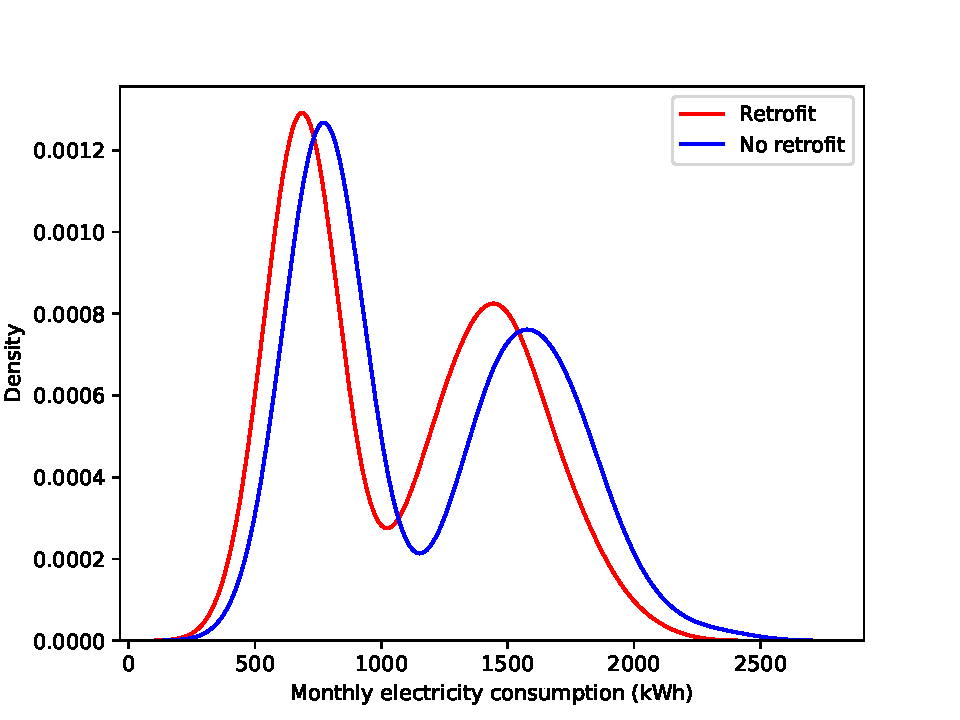
\includegraphics[scale = 0.6]{./figure/2_hist.pdf}
    \caption{Density plot of electricity consumption}
    \label{f1:hist}
\end{figure}

\subsection{OLS regression}
There are different computation methods to obtain the OLS estimates. I describe the method used to compute the OLS estimates inside the \verb!OLS.py! file within the \verb!manualOLS! class. The class takes three argument \verb!useRobust, addIntercept,! and \verb!method!. Options of \verb!method! to use are \verb|'byhand'| to use matrix inversion, \verb|'stasmodels'| to used the python canned routing, and \verb|'leastsquares'| to use the least square minimizer. The argument \verb!useRobust! is by default set to \verb!False! while \verb!addIntercept! is by default set to \verb!True!. User can use \verb!useRobust=True! to get the heteroscedasticity robust OLS standard error estimator. The class return the coefficient estimates under the properties \verb!.beta()!. The standard error of estimates can be obtained from the properties \verb!.beta_std()!. 

Table \ref{t2:ols} and \ref{t3:ols_robust} shows the estimates from using different computation method which gives identical coefficient estimates.

\begin{table}[H]\centering
\begin{threeparttable}
    \caption{OLS estimates for different computation methods}
    \label{t2:ols}
    \begin{tabular}{lccc}
\toprule
 & By Hand & Stats Model & Least Squares \\
\midrule
=1 if house received retrofit & -109.666 & -109.666 & -109.666 \\
  & (7.948) & (7.948) & (7.948) \\
Square feet of home & 0.615 & 0.615 & 0.615 \\
  & (0.006) & (0.006) & (0.006) \\
Outdoor average temperature (\textdegree F) & 3.255 & 3.255 & 3.255 \\
  & (1.924) & (1.924) & (1.924) \\
Constant & -83.603 & -83.603 & -83.593 \\
  & (154.360) & (154.360) & (154.360) \\
M.S.E. & 125.652 & 125.652 & 125.652 \\
\bottomrule
\end{tabular}

    \begin{tablenotes}
    \small \item The s.e. estimates is obtained using the square-root of the diagonal element of the following covariance matrix:
    \begin{align*}
        \hat{V}(\hat{\beta})=\frac{1}{n-k}\sum_{j=1}^k \underbrace{\hat{e}_j^2}_{y_i-\textbf{x}_i\hat{\beta}}\left(\textbf{X'}\textbf{X}\right)^{-1}
    \end{align*}
    
    \end{tablenotes}
\end{threeparttable}
\end{table}

\begin{table}[H]\centering
    \begin{threeparttable}
        \caption{OLS estimates with robust S.E. for different computation methods}
        \label{t3:ols_robust}
        \begin{tabular}{lccc}
\toprule
 & By Hand & Stats Model & Least Squares \\
\midrule
=1 if retrofit & -109.666 & -109.666 & -109.666 \\
  & (7.943) & (7.943) & (7.943) \\
Square feet of home & 0.615 & 0.615 & 0.615 \\
  & (0.007) & (0.007) & (0.007) \\
Outdoor average temperature & 3.255 & 3.255 & 3.255 \\
  & (1.932) & (1.932) & (1.932) \\
Constant & -83.603 & -83.603 & -83.593 \\
  & (154.695) & (154.695) & (154.695) \\
MSE & 125.652 & 125.652 & 125.652 \\
\bottomrule
\end{tabular}

        \begin{tablenotes}
        \small \item The s.e. estimates is obtained using the square-root of the diagonal element of the following covariance matrix:
    \begin{align*}
        \hat{V}(\hat{\beta})=\left(\textbf{X'}\textbf{X}\right)^{-1}\left(\frac{n}{n-k}\sum_{j=1}^k \hat{e}_j^2\textbf{x}_j\textbf{x}_j\right)\left(\textbf{X'}\textbf{X}\right)^{-1}    
        \end{align*}
        \end{tablenotes}
    \end{threeparttable}
    \end{table}

\section{Stata}

\subsection{Balance table}

\begin{table}[H]\centering
Table \ref{t4:balance} is produced from Stata and show exactly the same result as in Table \ref{t1:balance}.

\begin{threeparttable}
    \caption{Balance table from Stata}
    \label{t4:balance}
    {
\def\sym#1{\ifmmode^{#1}\else\(^{#1}\)\fi}
\begin{tabular}{l*{3}{c}}
\hline\hline
                    &\multicolumn{1}{c}{Control}&\multicolumn{1}{c}{Treatment}&\multicolumn{1}{c}{P-value}\\
\hline
Electricity         &    1181.33 &    1086.75 &       0.001\\
                    &   (454.31) &   (423.96) &     [3.404]\\
Square feet of home &    1633.05 &    1657.55 &       0.572\\
                    &   (682.90) &   (686.27) &    [-0.566]\\
Outdoor average temperature&      79.89 &      79.89 &       0.987\\
                    &     (2.16) &     (1.97) &    [-0.016]\\
\hline
Observations        &         501&         499&       1,000\\
\hline\hline
\end{tabular}
}

    \begin{tablenotes}
    \small \item \textit{Notes} Columns 1 and 2 report the mean and standard deviation in parentheses of the variables for the control group and treatment group consecutively. The third column show the p values for difference-in-means test and its corresponding t-statistics in square bracket.
    \end{tablenotes}
\end{threeparttable}
\end{table}

\subsection{Scatterplot}

\begin{figure}[H]
    \centering
    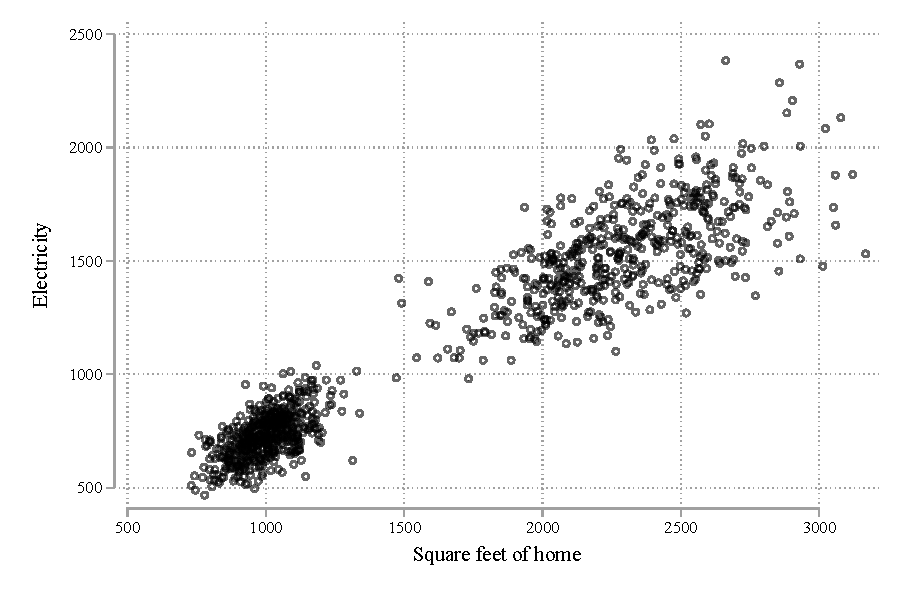
\includegraphics[scale = 1]{./figure/twoway.pdf}
    \caption{Scatterplot of electricity consumption and square feet of home}
    \label{f2:twoway}
\end{figure}

\subsection{OLS regression}
Table \ref{t5:ols_stata} is produced from Stata and shows the same result with the Python version.

\begin{table}[H]\centering
\begin{threeparttable}
    \caption{Estimates from Stata}
    \label{t5:ols_stata}
    \begin{tabular}{l*{2}{c}}
\hline\hline
                    &\multicolumn{1}{c}{OLS}&\multicolumn{1}{c}{OLS with robust s.e.}\\
\hline
=1 if house received retrofit&    -109.666&    -109.666\\
                    &     (7.948)&     (7.943)\\
Square feet of home &       0.615&       0.615\\
                    &     (0.006)&     (0.007)\\
Outdoor average temperature (\textdegree F)&       3.255&       3.255\\
                    &     (1.924)&     (1.932)\\
Constant            &     -83.603&     -83.603\\
                    &   (154.360)&   (154.695)\\
\hline
MSE                 &     125.652&     125.652\\
\hline\hline
\end{tabular}

    \begin{tablenotes}
    \small \item The non-robust and robust standard error estimates is exactly the same as in Table \ref{t2:ols} and \ref{t3:ols_robust}.
    \end{tablenotes}
\end{threeparttable}
\end{table}

\end{document}